Supervised Learning Machine Learning can be divided into two classes of problems, regression and classification. Where in Classification the machine learning algorithm should decide between discrete class labels, the output of a regression algorithm is usually a continuous quantity. Due to the nature of the Gaussian Processes suiting regression problems, a focus is put on these, even though Gaussian Processes can also solve classification problems \cite{Rasmussen_06}. There are several ways of interpreting a Gaussian process, the function space view, and the weight-space view. In the weigth space view, the Gaussian Process is pictured as a process, with infinity many basis functions with corresponding weights. In the function space view, the gaussian process is a distribution over functions, and inference takes place in the function space defined by the process. The Gaussian process, as mentioned in section \ref{sec:capm} and \ref{sec:apt}, is mainly used to find the covariance matrices, that encode the covariance structure of the problem. 

\subsubsection{Weight Space View}
A simple Gaussian process will be derived here. Starting with a standard linear regression model with Gaussian noise
\begin{subequations}%Linear Regression Gaussian
	\label{eq:Linear Regression Model}
	\begin{align}
	f(x) = \bm{x}^\top \bm{w}         \label{eq: linear regression function} \\
	y = f(\bm{x}) + \epsilon         \label{eq: observed target value} \\
	\epsilon \thicksim \mathcal{N}(0, \sigma_{n}^{2})
	\end{align}
\end{subequations}
Here $\bm{x}$ is the input vector, $\bm{w}$ is the vector containing the weigths, $f$ is the function value and $y$ the observed target value. Also, $\epsilon$ is the independent noise, and it follows an independent, identically distributed Gaussian distribution with zero mean and variance $\sigma_{n}^{2}$. The likelihood, as probability density of observations given parameters factors over the cases of the training set. 
\begin{subequations}%Likelihood in Weight Space View
	\label{eq:Likelihood Weight Space View}
	\begin{align}
	p(\bm{y}|X,\bm{w}) = \prod_{i=1}^{n} p(y_i|\bm{x}_{i}, \bm{w}) =  \prod_{i=1}^{n} \frac{1}{\sqrt{2\pi}\sigma_{n}} \exp \Big( -\frac{(y_i -\bm{x}_{i}^{\top}\bm{w})^2}{2\sigma^2_n}\Big)      \label{eq:likelihood wieght space 1} \\
	= \frac{1}{(2\pi\sigma_n^2)^{n/2}} \exp \Big( -\frac{1}{2\sigma_n^2 }|\bm{y}-X^{\top}\bm{w}|^2 \Big) = \mathcal{N}(X^{\top}\bm{w}, \sigma_n^2 I)         \label{eq:likelihood weight space 2}.
	\end{align}
\end{subequations}
$X$ is all the data points from the input, and $|x|$ stands for the euclidian length of a vector $x$. Also, a prior must be specified, containing our beliefs about the parameters before observing the input. Therefore, we will distribute the weights using a zero mean Gaussian prior with covariance matrix $\Sigma_p$, 
\begin{equation}%Weights Distribution
	\bm{w} \thicksim \mathcal{N}(\bm{0}, \Sigma_p).
\label{Distribution of weights using a zero mean Gaussian with covariance matrix.}
\end{equation}
To apply Bayes rule, we need a marginal likelihood, which acts as a normalizing constant, and is independent of the weights by integrating them out. 
\begin{equation}%marginal likelihood
	p(\bm{y}|X) = \int p(\bm{y}|X,\bm{w}) p(\bm{w}) d\bm{w}
\label{eq: Marginal likelihood as normalizing constant}
\end{equation}
The full Bayes rule in this case then becomes the following
\begin{equation}%Bayes Rule for Linear Regression
	p(\bm{w}|\bm{y},X) = \frac{p(\bm{y}|X,\bm{w})p(\bm{w})}{p(\bm{y}|X)}
\label{Bayes Rule for linear Regression}
\end{equation}
Using complete the square and ignoring the marginal likelihood, we find
\begin{equation}%unnormalized posterior
	p(\bm{w}|X,\bm{y}) \thicksim \mathcal{N}(\frac{1}{\sigma_n^2}(\frac{1}{\sigma_n^2}XX^{\top}+ \Sigma_p^{-1}), (\frac{1}{\sigma_n^2}XX^{\top}+ \Sigma_p^{-1})^{-1})
\label{Unnormalized posterior}
\end{equation}
With this, we can easily find the predictive distribution for $f_* \triangleq f(\bm{x}_*)$, by averaging the output of all possible linear models with respect to the Gaussian posterior,
\begin{subequations}%Gaussian posterior predictive distribution
	\label{eq:Gaussian posterior predictive distribution}
	\begin{align}
		p(f_*|\bm{x}_*,X,\bm{y}) = \int p(f_*|\bm{x}_*, \bm{w})p(\bm{w}|X,\bm{y}) d\bm{w}    \label{eq:predictive distribution 1} \\
		= \mathcal{N}(\frac{1}{\sigma_n^2}\bm{x}_*^{\top}(\frac{1}{\sigma_n^2}XX^{\top}+ \Sigma_p^{-1})^{-1}X\bm{y}, \bm{x}_*^{\top}(\frac{1}{\sigma_n^2}XX^{\top}+ \Sigma_p^{-1})^{-1}\bm{x}_*).         \label{eq: predicitve distribution 2}
	\end{align}
\end{subequations}
This model can easily be expanded by transforming the input into some high dimensional space using a set of basis functions and subsequently applying the linear model in this higher dimensional space. Applying the map $\phi(x) = (1,x,x^2,x^3,x^4,...)^{\top}$ would for example implement polynomial regression, during which a $D$-dimensional input vector $x$ is mapped into an $N$-dimensional feature space. This allows us to rewrite the model as
\begin{subequations}%Feature Space Gaussian process
	\label{eq:Feature Space Gaussian process}
	\begin{align}
	f(\bm{x}) = \phi(\bm{x})^{\top} \bm{w}         \label{eq: feature space model} \\
	f_*|\bm{x}_*,X,\bm{y}  \thicksim \mathcal{N}\Big( \frac{1}{\sigma_n^2}\phi(\bm{x}_*)^{\top}(\sigma_n^{-2}\Phi \Phi^{\top} + \Sigma_p^{-1})^{-1} \Phi \bm{y} , \label{eq: predictive distribution mean} \\
	 \phi(\bm{x}^{\top})(\sigma_n^{-2}\Phi \Phi^{\top} + \Sigma_p^{-1})^{-1} \phi(\bm{x}_*) \Big)        \label{eq: predictive distribution covariance} 
	\end{align}
\end{subequations}
where $\Phi(X)$ is the aggregation of all columns $\phi(\bm{x})$ for all cases in the data set in the transformed space. It presents a computational time benchmark when executing such a model, since the inversion of $N\times N$ matrices is of $\mathcal{O}(N^3)$ complexity. With high-dimensional feature spaces, reducing the argument of the complexity function is valuable. So, sometimes rewriting the equations as
\begin{equation}%rewritten Feature Space Gaussian Process evaluated in data space. 
	f_*|\bm{x}_*,X,\bm{y} \thicksim \mathcal{N}\Big( \phi_*^{\top}\Sigma_p\Phi(K+ \sigma_n^2 I)^{-1}\bm{y}, \phi_*^{\top} \Sigma_p \phi_* - \phi_*^{\top} \Sigma_p \phi_*(K+ \sigma_n^2 I)^{-1}\phi_*^{\top} \Sigma_p \phi_* \Big)
\label{Rewritten Feature Space Gaussian Process evaluated in data space.}
\end{equation}
is useful, since the complexity $\mathcal{O}(n^3)$ is the maximum complexity possible for $n$ datapoints \cite{Rasmussen_06}. Then, the kernel function $k(\bm{x},\bm{x'}) = k(\cdot , \cdot) = \phi_*^{\top} \Sigma_p \phi_*$ is easily identified. The kernel is often also called covariance function. \newline

\subsubsection{Function Space View}
This derivation can also be done in function space. Here, we can define a Gaussian Process as a collection of random variables, any finite number of which have a joint Gaussian distribution. Since a Gaussian process is solely defined by its mean and kernel function, it can be written as
\begin{subequations}%Gaussian process function space view
	\label{eq:Gaussian_process_function_space_view}
	\begin{align}
	m(x) =\mathbb{E}[f(x)]         \label{eq:function space view mean} \\
	k(\bm{x},\bm{x'}) = \mathbb{E}[(f(\bm{x})-m(\bm{x}))(f(\bm{x'})-m(\bm{x'})))]         \label{eq:function space view covariance function} \\
	f(x) \thicksim \mathcal{GP}(m(\bm{x}), k(\bm{x}, \bm{x'})).               \label{fuinction space view gaussian process}
	\end{align}
\end{subequations}
The Function space view notation will be the notation further on used in this thesis. Here, $\mathcal{GP}$ stands for a Gaussian Process, $m(\bm{x})$ is the mean function, and $k(\bm{x}, \bm{x'})$ is the kernel function. The consistency requirement, also marginalization property, states, that for a $\mathcal{N}$ $(y_a, y_b) \thicksim \mathcal{N}(\bm{\mu}, \Sigma)$ with general mean vector $\bm{\mu} = (m(\bm{x}_a), m(\bm{x}_b))^{\top}$ and covariance matrix $\Sigma$, the underlying $\mathcal{N}(y_a)$ is specified by $y_a \thicksim \mathcal{N}(\mu_a, \Sigma_{aa})$. $\Sigma_{aa}$ then is the submatrix of $\Sigma$ relevant to the distribution for $y_a$. Since the submatrixes are not intertwined in $\Sigma$, the examination of a larger set of variables does not change the distribution of a subset. Using the previously discussed linear regression model $f(x) = \phi(\bm{x})\bm{w}^{\top}$ with a gaussian prior on $\bm{w}$ we have mean and covariance
\begin{subequations}%Function space view linear regression mean and covariance
	\label{eq:Function space view linear regression mean and covariance}
	\begin{align}
	\mathbb{E}[f(\bm{x})] = \phi(\bm{x})^{\top} \mathbb{E}[\bm{w}] = 0         \label{eq:function space linear mean} \\
	\mathbb{E}[f(\bm{x})f(\bm{x'})] = \phi(\bm{x})^{\top} \mathbb{E}[\bm{w}\bm{w}^{\top}]\phi(\bm{x}) = \phi(\bm{x})^{\top}\Sigma_p\phi(\bm{x'}).         \label{eq:function space linear covariance}
	\end{align}
\end{subequations}
Given a kernel function, we can generate a random sample from a GP with Covariance matrix $K(X_*, X_*)$, where $X_*$ is the matrix containing all input points. 
\begin{equation}%Random Gaussian prior samples
	\bm{f_*} \thicksim \mathcal{N}(\bm{0}, K(X_*, X_*))
\label{Random Gaussian vector}
\end{equation}
The most used kernel function is the squared exponential,
\begin{equation}%squared exponential
	k_{sqe}(\bm{x_i}, \bm{x_j}) = exp(-\frac{1}{2l^2}d_{ij}^2).
	\label{eq:squared-exponential}
\end{equation}
Incorporating the knowledge of the training data for noise free predictions then leads us to
\begin{equation}%Joint Distribution according to prior
	\begin{bmatrix}	\bm{f} \\ \bm{f_*} \end{bmatrix} \thicksim \mathcal{N} \Bigg(0, \begin{bmatrix} K(X,X) & K(X,X_*) \\ K(X_*,X) & K(X_*,X_*) \end{bmatrix} \Bigg),
\label{eq:joint_distribution_according_to_prior}
\end{equation}
where now all variables without $_*$ are training variables, and all variables with $_*$ are the respective test variables. This gives 
\begin{equation}%conditioned/joint Gaussian prior
	\bm{f}_*|X_*,X,\bm{f} \thicksim \mathcal{N}(K(X_*,X)K(X,X)\bm{f}, K(X_*,X_*)-K(X_*,X)K(X,X)^{-1}K(X,X_*))
\label{conditioned/joint Gaussian prior}
\end{equation}
for the conditioned, joint Gaussian prior distribution on observations. Extending the model to incorporate noise on the data, we find
\begin{equation}%Joint Gaussian distribution according to prior with noise
	\begin{bmatrix}	\bm{y} \\ \bm{f_*} \end{bmatrix} 
	\thicksim \mathcal{N} \Bigg(0, 
	\begin{bmatrix} K(X,X)+\sigma_n^2 I & K(X,X_*) \\ K(X_*,X) & K(X_*,X_*) \end{bmatrix} \Bigg),
\label{eq:joint_gaussian_distribution_according_to_prior_with_noise}
\end{equation}
where the key predictive equations for Gaussian process regression are
\begin{subequations}%Key predictive equations for Gaussian process regression
	\label{eq: Key predictive equations for Gaussian process regression}
	\begin{align}
	\bm{f}_*|X,\bm{y},X \thicksim \mathcal{N}(\overline{\bm{f}_*}, cov(\bm{f}_*)),         \nonumber \\
	\overline{\bm{f}_*} \triangleq \mathbb{E}[\bm{f}_*|X,\bm{y},X_*] = K(X_*,X)[K(X,X) + \sigma_n^2 I]^{-1}\bm{y},        \nonumber \\
	cov(\bm{f_*}) = K(X_*,X_*) - K(X_*,X)[K(X,X)+ \sigma_n^2 I]^{-1}K(X,X_*).       
	\end{align}
	\label{eq:Key_predictive_equations_for_GP_reg}
\end{subequations}
Introducing the marginal likelihood $p(\bm{y}|X)$ again, we find
\begin{equation}%Marginal Likelihood function space view
	p(\bm{y}|X) = \int p(\bm{y}|\bm{f},X) p(\bm{f}|X) d\bm{f}.
\label{eq:marginal_likelihood_function_space_view}
\end{equation}
Solving this integral analytically it results to
\begin{equation}%Log Marginal likelihood
	log \Big(p(\bm{y}|X)\Big) = -\frac{1}{2}\bm{y}^{\top}(K+ \sigma_n^2 I)^{-1}\bm{y} -\frac{1}{2}log|K+ \sigma_n^2 I| - \frac{n}{2}log ( 2\pi).
\label{eq:Log_marginal_likelihood}
\end{equation}
Using this, we have derived the regular Gaussian process. It is easy to see, that iterative usage of the learning equations (previously: key predictive equations) is the same as learning from all data points at once due to the marginalization property. The following figures provide an example. At first, we introduce random prior samples  in figure \ref{fig:prior_squ_exp}, specified by a squared exponential kernel centered around a mean of 0 and with a covariance of 2. 
\begin{figure}[h!]%prior example squared exponential
	\centering
	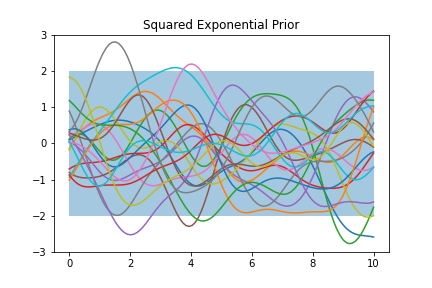
\includegraphics[width=4in]{img/05_3/gp_prior.png}
	\caption[GP prior samples]
	{Samples from a Gaussian Process prior with a squared exponential kernel. To add to the draws, the 95\% confidence interval is highlighted with a blue background. }
	\label{fig:prior_squ_exp}
\end{figure}
Then, we introduce data points, which were randomly generated using a modified sine function with added gaussian noise, see figure \ref{fig:generated_data}. 
\begin{figure}[h!]%data points to train on
	\centering
	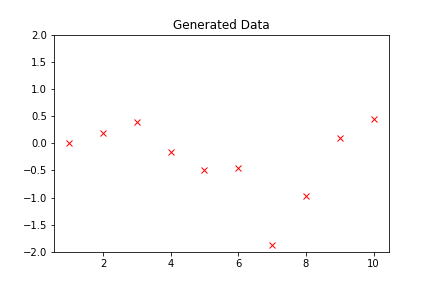
\includegraphics[width=4in]{img/05_3/generated_data.png}
	\caption[Random data from sine function with Gaussian noise]
	{Data generated from a sine function with added Gaussian noise.}
	\label{fig:generated_data}
\end{figure}
Using the learning equations \ref{eq:Key_predictive_equations_for_GP_reg}, we can train a Gaussian process on the data points and find the following posterior samples, see figure \ref{fig:GP_sqexp_samples} and confidence intervals, having solved the Gaussian Process. 
\begin{figure}[h!]
	\centering
	\begin{minipage}{0.45\textwidth}
		\centering
		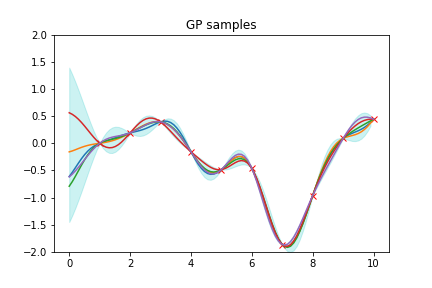
\includegraphics[scale=0.6]{img/05_3/gp_samples.png} % first figure itself
		\caption[Trained GP samples with covariance interval]{The GP conditioned on the generated dataset, with the 95\% confidence interval and 5 samples drawn from the GP. }
		\label{fig:GP_sqexp_samples}
	\end{minipage}\hfill
	\begin{minipage}{0.45\textwidth}
		\centering
		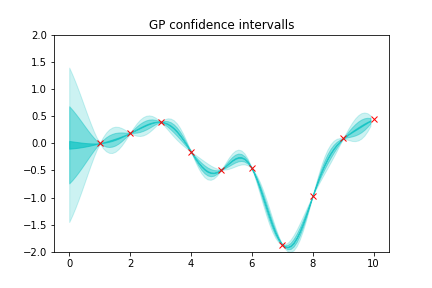
\includegraphics[scale=0.6]{img/05_3/gp_confints.png} % second figure itself
		\caption[Trained GP with covariance intervals]{The GP conditioned on the generated dataset, with confidence intervals drawn into the graph as blue shading. }
		\label{fig:GP_confidence_intervals}
	\end{minipage}
\end{figure}
The confidence intervals in figure \ref{fig:GP_confidence_intervals} have 1, 2, and 3 $\sigma$. This depiction also highlights the interpretation of GP predictions as probability distributions. \newpage